\section{Introduction}\label{sec:introduction}
The advent of Pre-trained Language Models (PLMs) has marked a transformative shift in the field of Natural Language Processing (NLP), offering versatile solutions across various applications \citep{he2021debertav3, lewis2019bart, touvron2023llama}. They have showcased unparalleled proficiency in executing a variety of language tasks, including Natural Language Understanding (NLU) and Natural Language Generation (NLG). These models typically have millions or even billions of parameters, necessitating substantial computational and memory requirements.
% For example, LLaMA consists of up to 70 billion parameters and GPT-3 comprises up to 175 billion parameters. 
However, the extensive computational and memory demands of these models pose significant challenges, especially in real-world deployments where resources are often constrained and need to be shared among many users.
% Basically, two obstacles are in the way: the model size and the substantial associated training cost, such as gradient and optimization cache.

To mitigate the extensive storage requirements of pre-trained models, quantization serves as a pivotal compression technique \citep{zafrir2019q8bert,  shen2020q, bai2022towards, dettmers2022llm}, converting high-precision numerical values into a discrete set of values. 
Typically, model parameters, originally stored in a 16-bit float format, are transformed into a 4-bit integer format through quantization, resulting in a substantial 75\% reduction in storage overhead.
Additionally, to facilitate the adaptation of quantized pre-trained models to downstream tasks efficiently, Low-Rank Adaptation (LoRA) is a viable approach \citep{hu2021lora}. This technique is a parameter-efficient fine-tuning method traditionally applied to high-precision pre-trained models. It is based on the hypothesis that the differences between fully fine-tuned weights and pre-trained weights exhibit low-rank properties. This allows these differences to be represented using low-rank matrices. As a result, the original pre-trained weights remain unaltered, with adaptations confined solely to these low-rank matrices, enabling effective task adaptation.
% A prominent technique within the realm of quantization is Quantization-Aware Training (QAT), initially quantizes a pre-trained model and subsequently fine-tunes the quantized model on downstream tasks. 
% Even though a variety of quantization methods have been proposed to approximate the original high-precision numbers as much accurate as possible, it inevitably introduces a certain level of errors, which yield significant deviation from the original model. 


% It usually attains higher accuracy on downstream tasks compared to other quantization methods, such as post-training quantization.

% There are two major quantization approaches: Quantization-Aware Training (QAT) and Post-Training Quantization (PTQ). QAT first quantizes a pre-trained model and then fine-tunes the quantized model on downstream tasks. By contrast, PTQ calibrates a pre-trained model by a small subset of fine-tuning data and then quantizes the model based on the calibration results. 

When quantizing pre-trained models, practitioners often concentrate primarily on the quantization technique, inadvertently neglecting the importance of subsequent LoRA fine-tuning  \citep{dettmers2023qlora, diao2023lmflow}.
For example, QLoRA inherits the fixup initialization \citep{zhang2019fixup} used in LoRA, which  \citep{dettmers2023qlora} attaches zero initialized low-rank adapters (see Section \ref{sec:background_lora}) to the quantized pre-trained model. The inevitable discrepancy introduced by quantization during the approximation of the original high-precision numbers, a scenario particularly pronounced in low-bit situations such as the 2-bit regime, can adversely impact the initialization of LoRA fine-tuning. As illustrated in Figure \ref{fig:quant_degrad_pretrain}, the quantized pre-trained model obtained by QLoRA exhibits severe degradation below the 3-bit level. This deviation in initialization often results in an inferior fine-tuning performance. As illustrated in Figure \ref{fig:quant_degrad_ft}, the fine-tuning performance drops as the quantization bit decreases when applying QLoRA. Moreover, it is noteworthy that QLoRA fails below the 3-bit level.

In this paper, we introduce a novel quantization framework, called \textbf{Lo}RA-\textbf{F}ine-\textbf{T}uning-aware \textbf{Q}uantization (LoftQ). It is designed specifically for pre-trained models that require quantization and LoRA fine-tuning.
This framework actively integrates low-rank approximation, working in tandem with quantization to jointly approximate the original high-precision pre-trained weights. This synergy significantly enhances alignment with the original pre-trained weights as illustrated in Figure~\ref{fig:quant_error}. 
Consequently, our method provides an advantageous initialization point for subsequent LoRA fine-tuning, leading to improvements in downstream tasks.
\begin{figure}[htb!]
\centering
\begin{subfigure}{0.46\columnwidth}
    \centering
    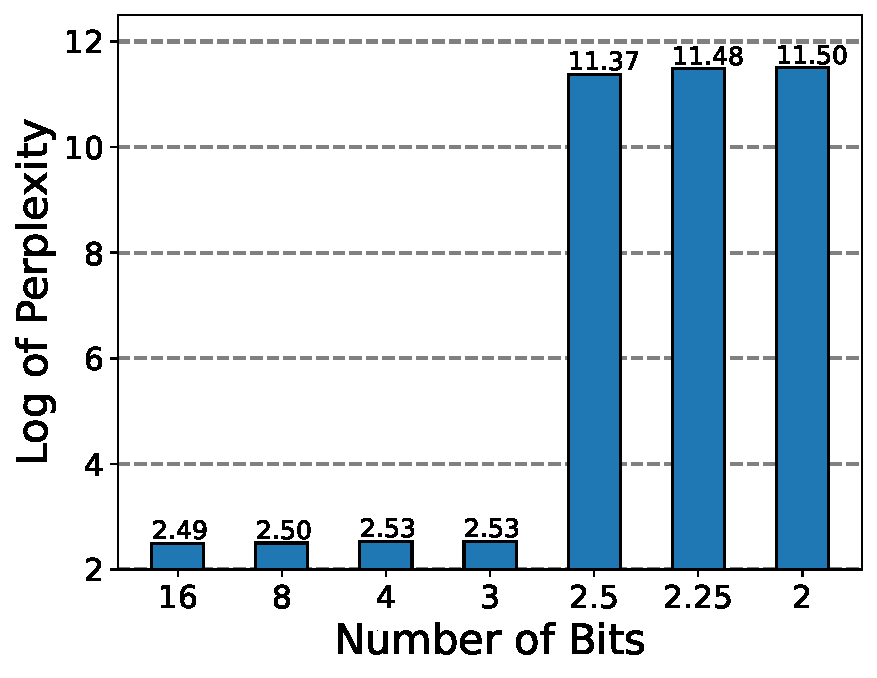
\includegraphics[width=1.0\textwidth]{figures/perplexity_bits_eval.pdf}
    \vspace{-5mm}
    \caption{Pre-trained LLAMA-2-13b on WikiText-2
    \label{fig:quant_degrad_pretrain}}
\end{subfigure}
\begin{subfigure}{0.46\columnwidth}
    \centering
    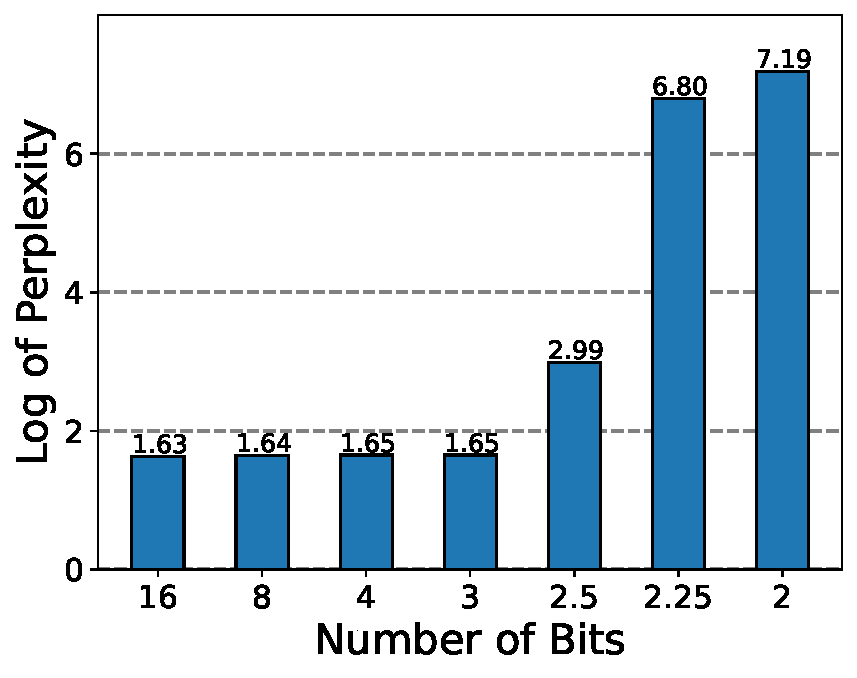
\includegraphics[width=1.0\textwidth]{figures/perplexity_bits_ft.pdf}
    \vspace{-5mm}
    \caption{Fine-tuned LLAMA-2-13b on WikiText-2
    \label{fig:quant_degrad_ft}}
\end{subfigure}
\vspace{-2mm}
\caption{QLoRA performance with different bits. {\bf Left:} QLoRA initialization of LLAMA-2-13b on WikiText-2. {\bf Right:} Apply QLoRA to LLAMA-2-13b on WikiText-2 language modeling task. Smaller perplexity indicates better performance.
\vspace{-3mm}
}
\end{figure}
% The low-rank adapters not only mitigate the gap between the quantized and full-precision weights, but also provide a better starting point for LoRA fine-tuning, compared to QLoRA \citep{dettmers2023qlora}, which employs a random initialization for low-rank adapters.
% Downstream task performance will benefit from this aligned initialization, based on the intuition from out pilot experiment results in Figure XX, that the closer the LoRA initialization aligns with the pre-trained model, the more significant the improvement in downstream task performance will be.


% It is natural to combine quantization and LoRA to achieve memory-saving and parameter-efficient fine-tuning. However, such naive combination confronts one major issue. 
% That is, quantization inevitably introduces a certain level of errors when approximating the original high-precision numbers, especially in low bit regimes, such as the 2-bit scenario. These quantization errors yield significant deviation from the original pre-trained model and thereby change the starting point of LoRA fine-tuning as well. Such deviation of LoRA initialization adversely impacts fine-tuning performance on downstream tasks (See Figure XX). 

% \citep{wu2022noisytune}
% Secondly, fine-tuning a quantized model remains a a challenge due to the discrete nature of quantization. Current optimization methods, like Stochastic Gradient Descent (SGD), struggle with the inability to update parameters in the discrete domain effectively. Even though one can apply SGD to the dequantized model and re-quantize it in each iteration, the training cost remains prohibitively high due to the comparable size of the gradient and optimization cache with the entire model.

% To mitigate the aforementioned quantization discrepancy, we propose \textbf{Lo}RA-\textbf{F}ine-\textbf{T}uning-aware \textbf{Q}uantization (LoftQ), which incorporates alternating quantization and low-rank approximation. Our method makes the hybrid approximation, i.e., the quantized weight plus the low-rank approximation, close to the full-precision pre-trained weight.
% Such alignment provides a better initialization for LoRA fine-tuning, compared to QLoRA \citep{dettmers2023qlora}, which employs a random initialization for low-rank adapters.
% We draw the intuition from our pilot experiment results in Figure XX, that the closer the LoRA initialization aligns with the pre-trained model, the more significant the improvement in downstream task performance will be.

% compared to QLoRA \citep{dettmers2023qlora}, which employs a random initialization for low-rank adapters.

% From the pilot experiment results (see Figure XX) that the closer the LoRA initialization is to the pre-trained model, the better downstream task performance is, our initialization is better than QLoRA \citep{dettmers2023qlora} that uses random initialization for low-rank adapters. 
 
% Thus, we need to enforce the initialization as close to the pre-trained high-precision weights as possible. 


% Therefore, we propose \textbf{Lo}RA-\textbf{F}ine-\textbf{T}uning-aware \textbf{Q}uantization (LoftQ), which quantizes a pre-trained model and updates the model by LoRA fine-tuning. In essence, it preserves the quantized pre-trained weights in a fixed state while directing all updates to the low-rank adapters during fine-tuning. {\OurAlg} thereby avoids updating the quantized weights, which sidesteps the issue that quantized weights are difficult to fine-tune. It further reduces the training cost because the trainable parameters are now restricted in those low-rank adapters, far less than the entire model. 
   
% Furthermore, {\OurAlg} initializes low-rank adapters by approximating the residual between the quantized weights and the original high-precision weights, which mitigates the quantization discrepancy. This mitigation helps to improve the downstream performance compared to QLoRA that use random initialization for low-rank adapters. Our pilot experiments (See Figure X) show that downstream task performance drops drastically if LoRA initialization does not align to pre-trained weights. Thus, we need to enforce the initialization as close to the pre-trained high-precision weights as possible. From fig, we can see \OurAlg successfully reduces the discrepancy between the original pretrained weights and the sum of quantized weights and low rank adapters through (iterative?) approximation of quantization residual.

We evaluate our quantization framework by conducting extensive experiments on downstream tasks, such as NLU, question answering, summarization, and NLG. 
Experiments show that {\OurAlg} consistently outperforms QLoRA across all precision levels. For instance, with 4-bit quantization, we achieve a 1.1 and 0.8 gain in Rouge-1 for XSum \citep{Narayan2018xsum} and CNN/DailyMail \citep{hermann2015teaching}, respectively. {\OurAlg} excels particularly in low-bit scenarios and works effectively with different quantization methods. For example, we achieve over an 8\% gain on MNLI \citep{wang2018glue} and more than 10\% on SQuADv1.1 \citep{rajpurkar-etal-2016-squad} with both 2-bit NormalFloat and the 2-bit uniform quantization. We have not seen our approach performs worse than QLoRA.


\begin{figure}[htb!]
\centering
\begin{subfigure}{0.48\columnwidth}
    \centering
    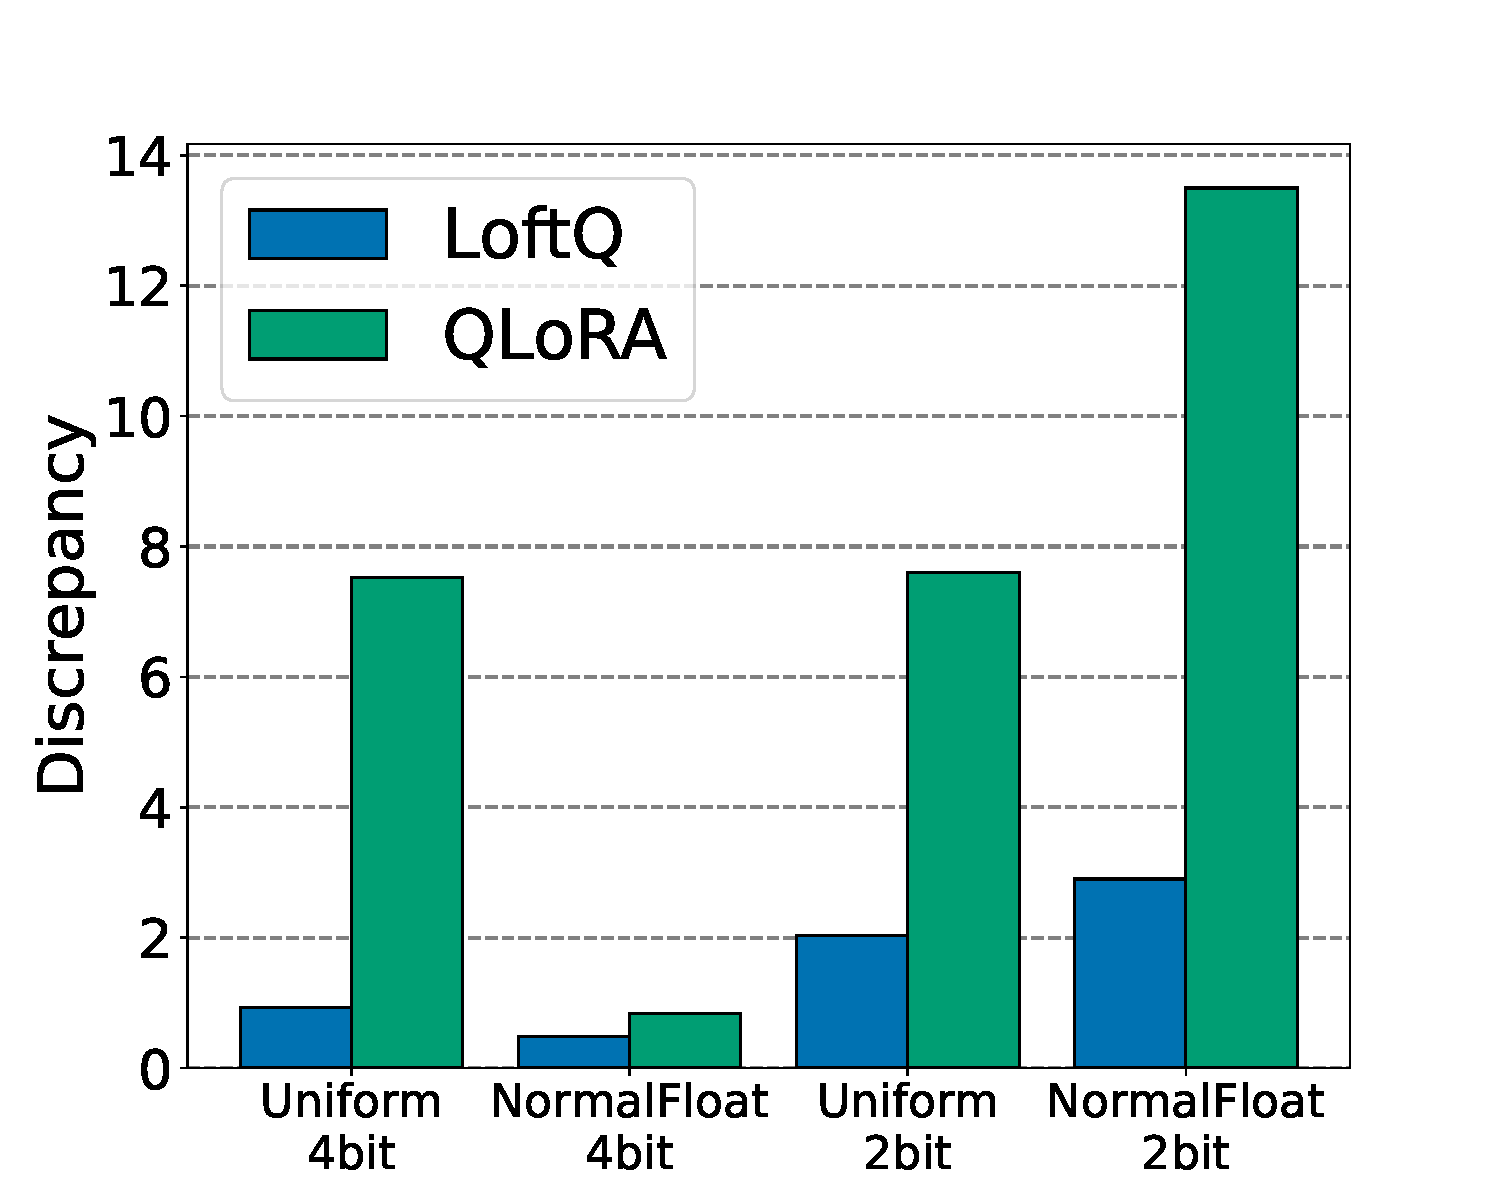
\includegraphics[width=1.0\textwidth]{figures/bart4_fc1_layer0.pdf}
    \vspace{-5mm}
    \caption{Spectral norm of the initialization difference}
\end{subfigure}
\begin{subfigure}{0.48\columnwidth}
    \centering
    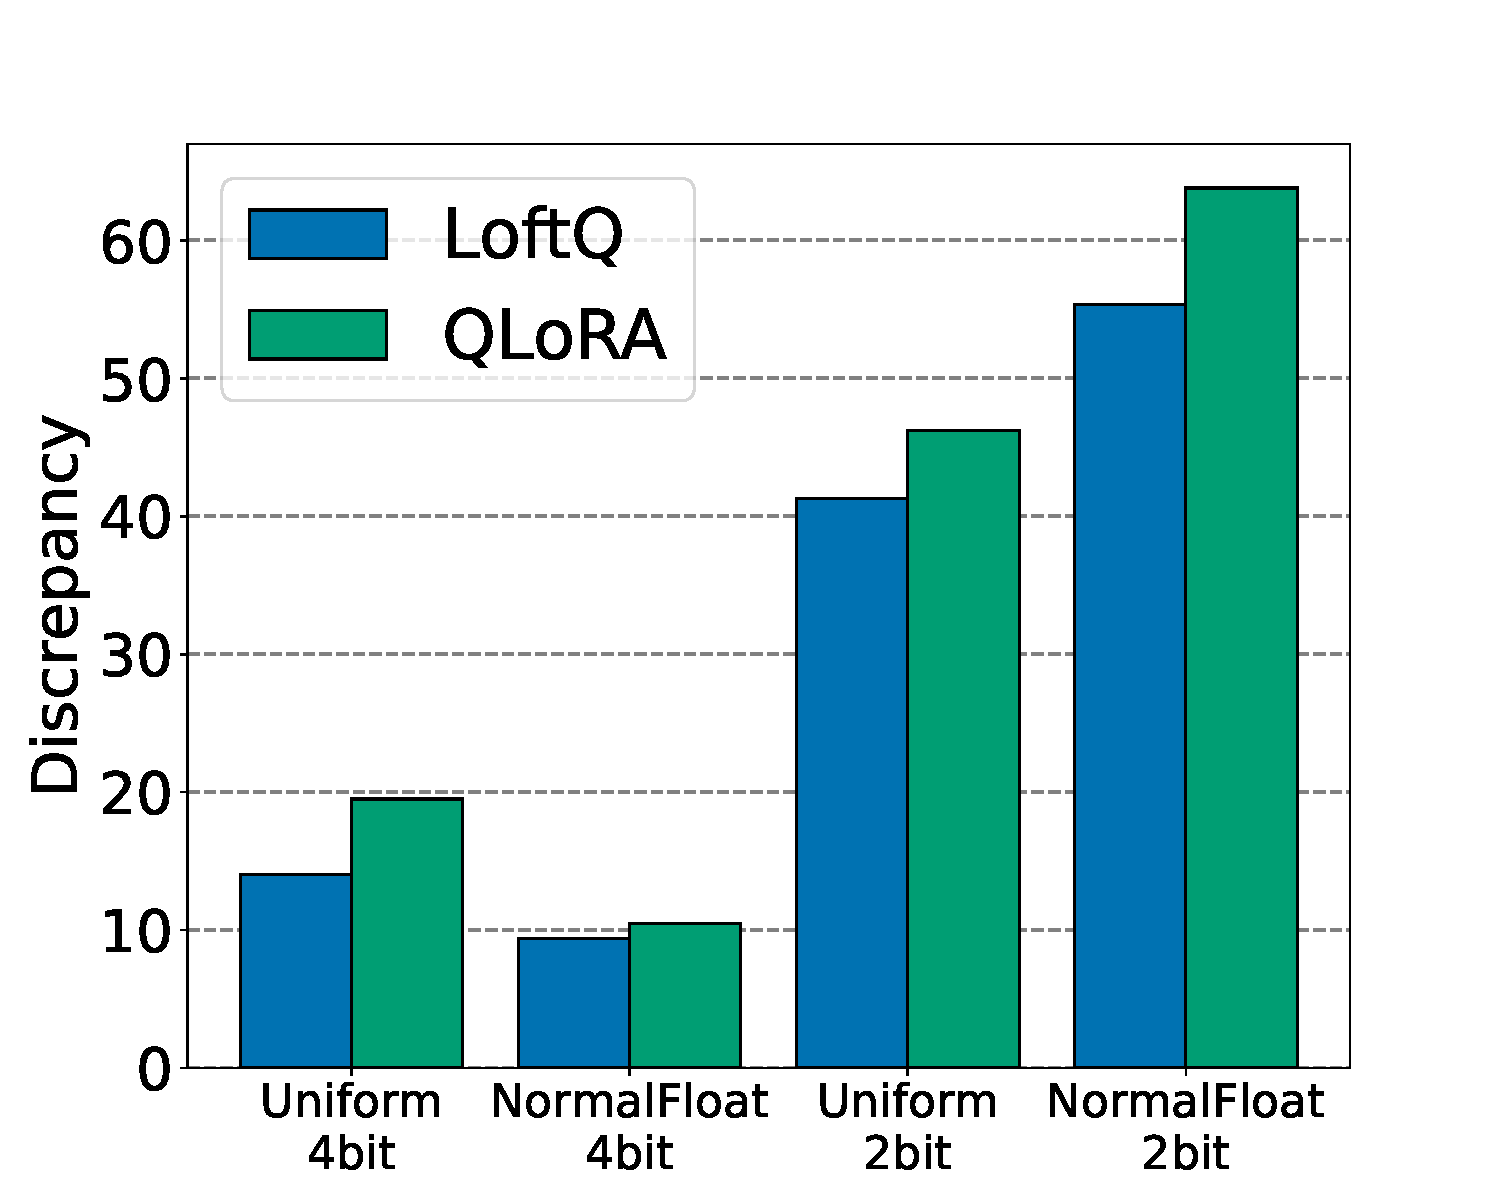
\includegraphics[width=1.0\textwidth]{figures/bart3_fc1_layer0.pdf}
    \vspace{-5mm}
    \caption{Frobenius norm of the initialization difference}
\end{subfigure}
\vspace{-1mm}
\caption{
Initialization discrepancy between the LoRA initialization and the original pre-trained weight matrix, described by the spectral norm and Frobenius norm of the difference. The weight matrix in the above figures is randomly selected in BART-large. The initialization is obtained by QLoRA and {\OurAlg}, with Uniform and NormalFloat quantization methods applied at both 2-bit and 4-bit levels. {\OurAlg} successfully mitigates the discrepancy, especially at the 2-bit level.
% Importance scores are calculated when compressing DeBERTa-base on SST-2 at the 3156\textsuperscript{th} step. \textit{Layer 7, Query} indicates the matrix is from the query matrix at the 7th layer.
}
\vspace{-1mm}
\label{fig:quant_error}
\end{figure}
 

% \textbf{Pruning} is also widely used to reduce the model size. It removes redundant parameters based on the importance score, for example, magnitude \citep{han2015learning}, sensitivity \citep{sanh2020movement, molchanov2019importance}, and uncertainty \citep{zhang2022platon}. However, when subjected to extreme high compression rates, such as removing more than 80\% parameters, the performance will demonstrate notable degradation. 
% We will compare our quantization method with the state-of-the-art pruning method \citep{li2023losparse} in Section \ref{sec:experiment}.\red{(need to mentioned it?)}
